\section{Results and Discussions}
\label{sec:results}

\begin{figure*}
	\centering
	\textbf{\em  4-class pair-level results. \quad\quad \quad            6-class pair-level results.    \quad      \quad\quad    13-class pair-level results}\vspace{-1.0cm}\\
	\subfigure{
		\begin{minipage}{0.25\linewidth}
			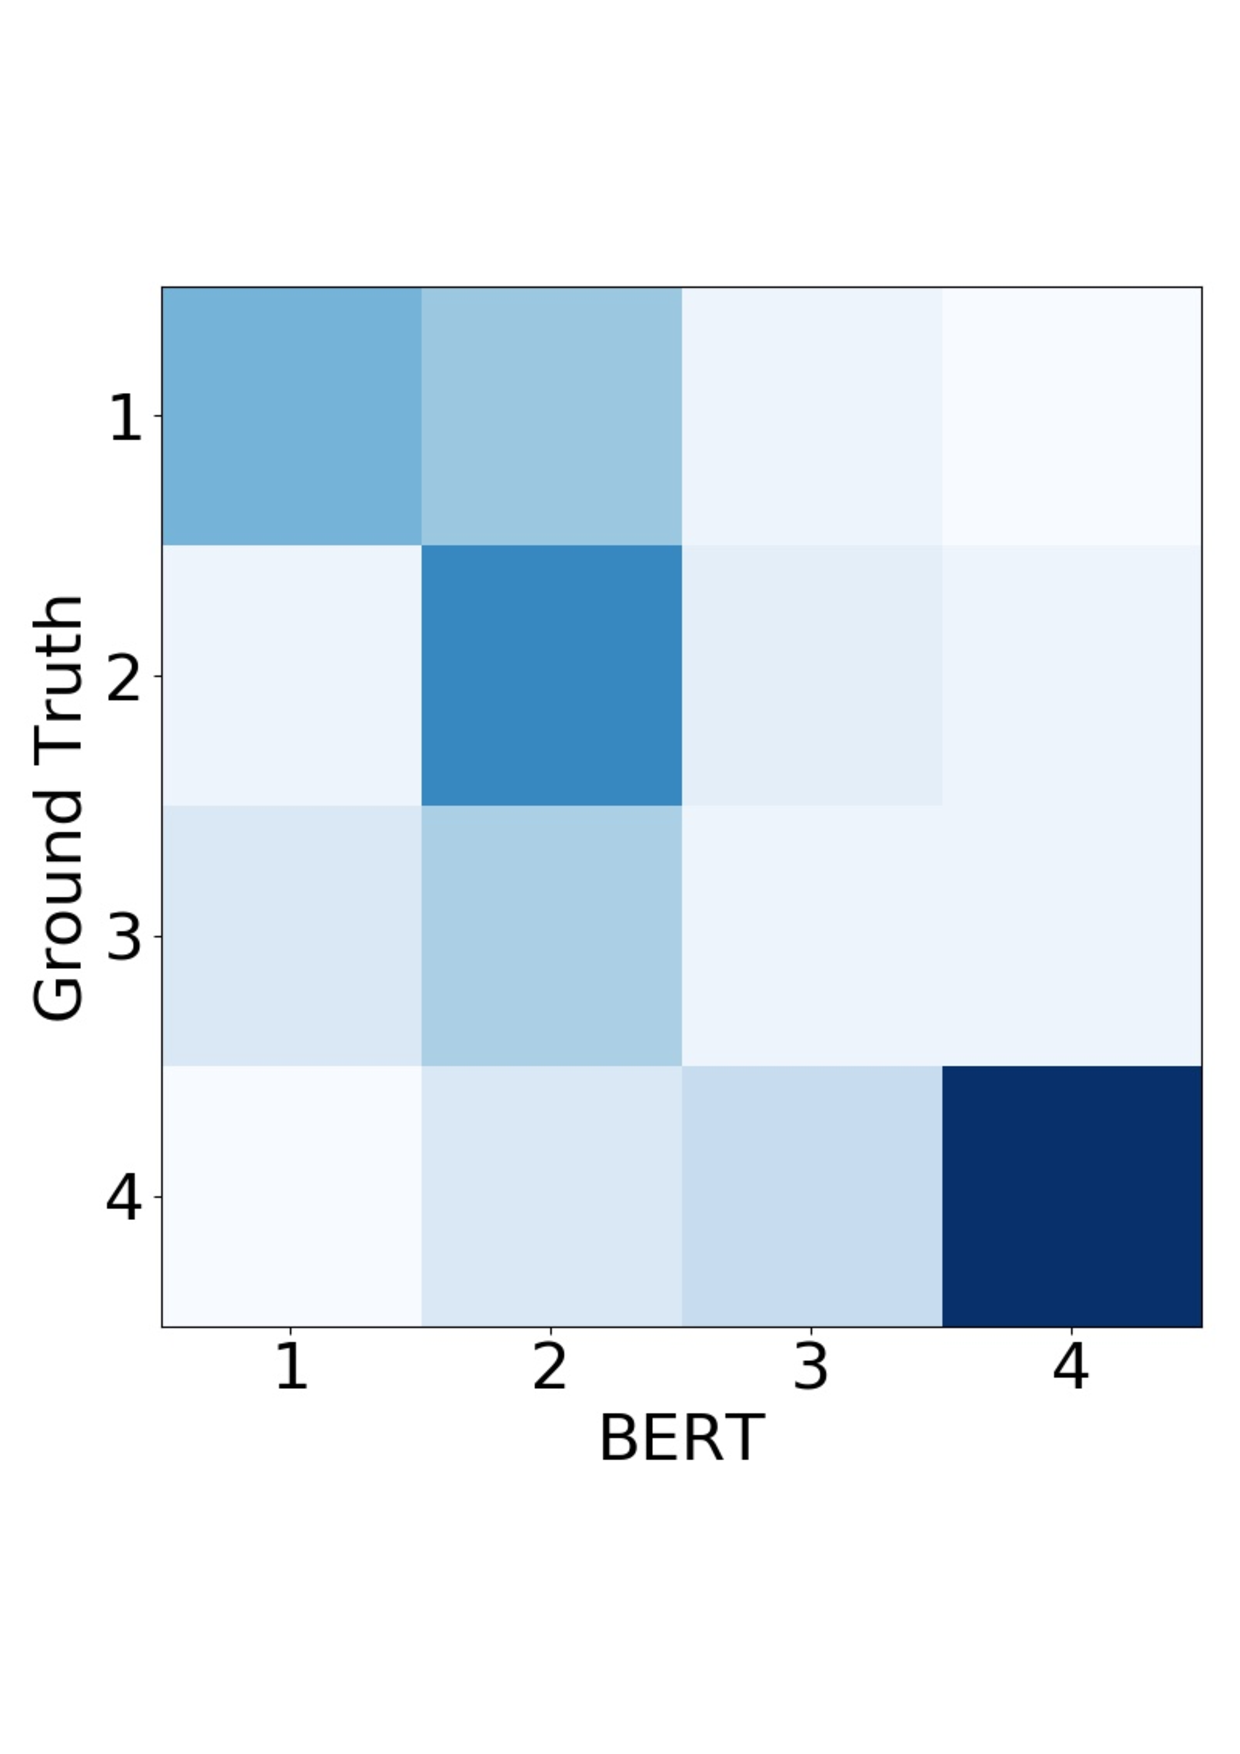
\includegraphics[width=1\linewidth]{BERT_4_pair}\vspace{-1.75cm}
			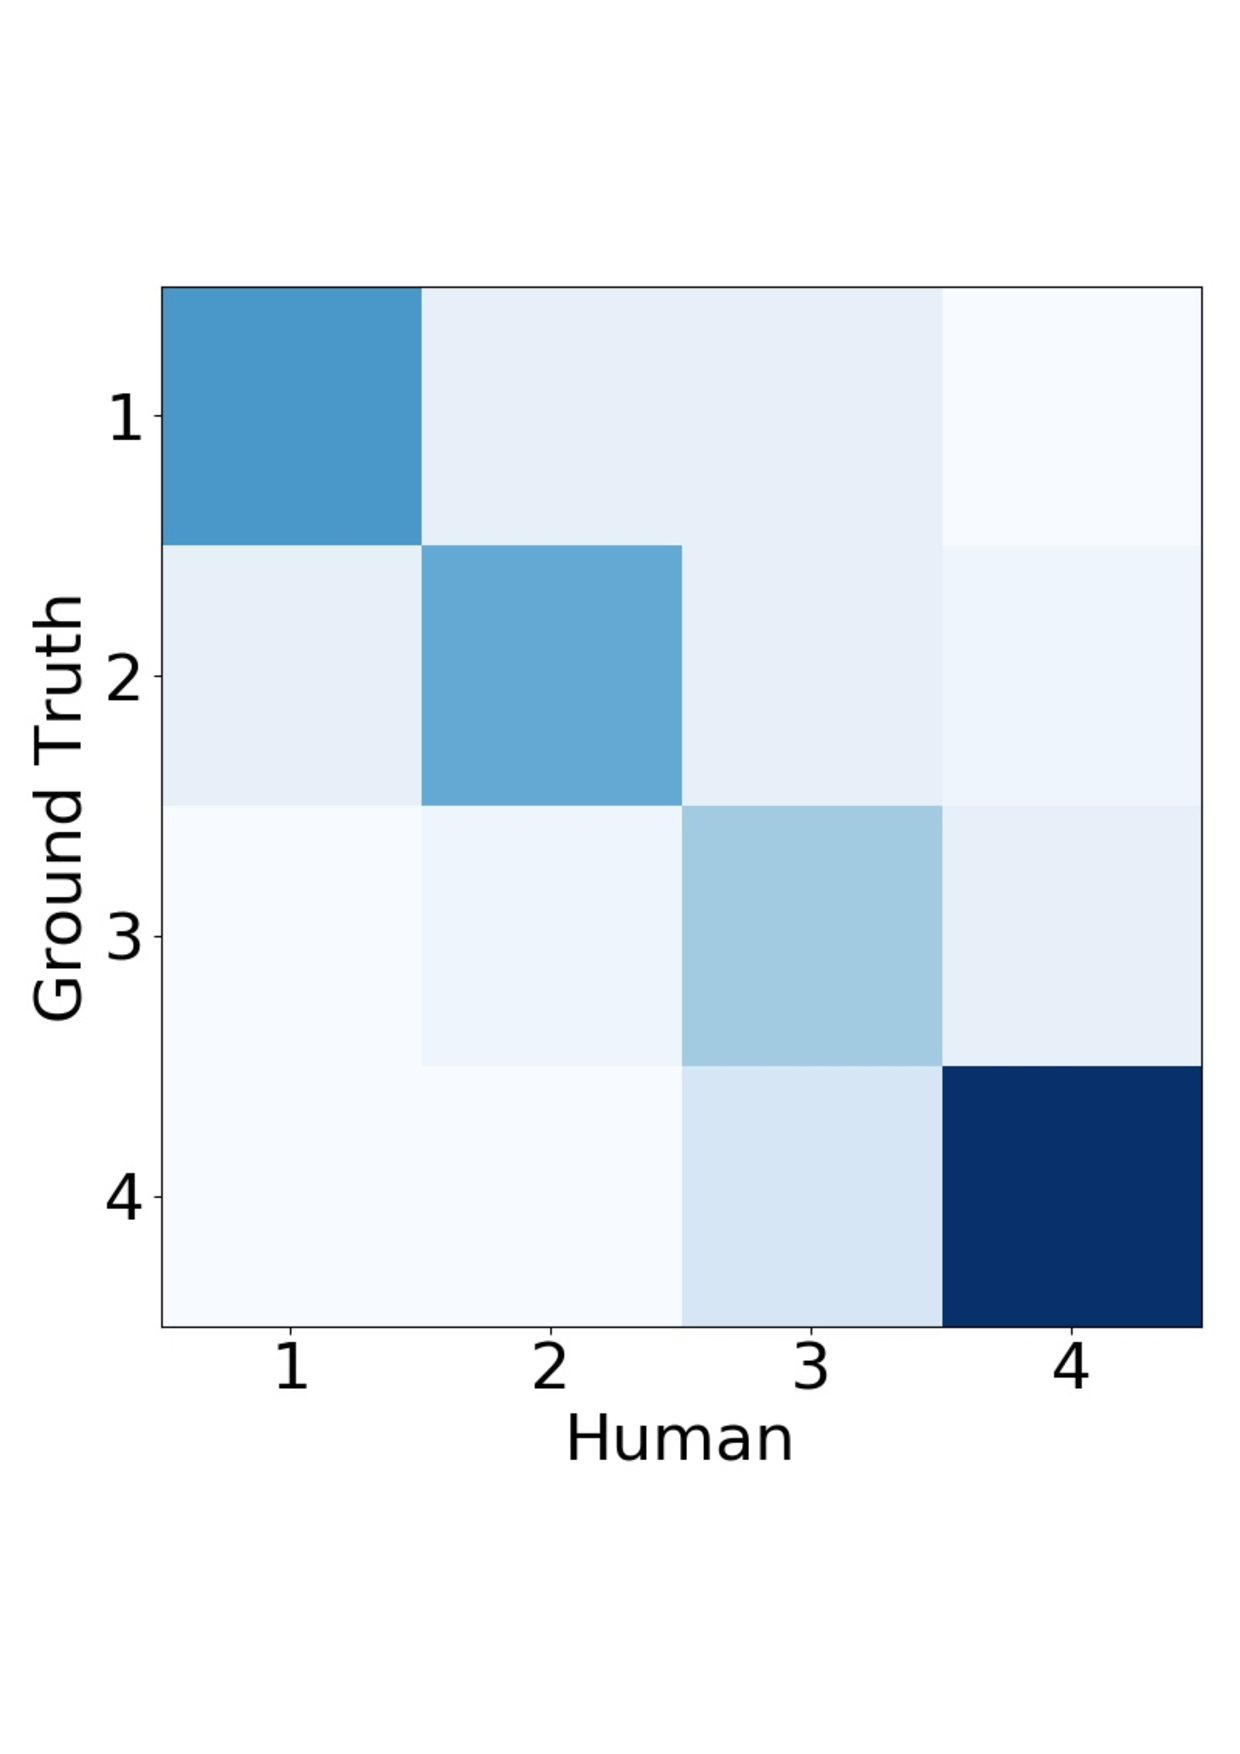
\includegraphics[width=1\linewidth]{human_4_pair}
	\end{minipage}}
	\subfigure{
		\begin{minipage}{0.25\linewidth}
			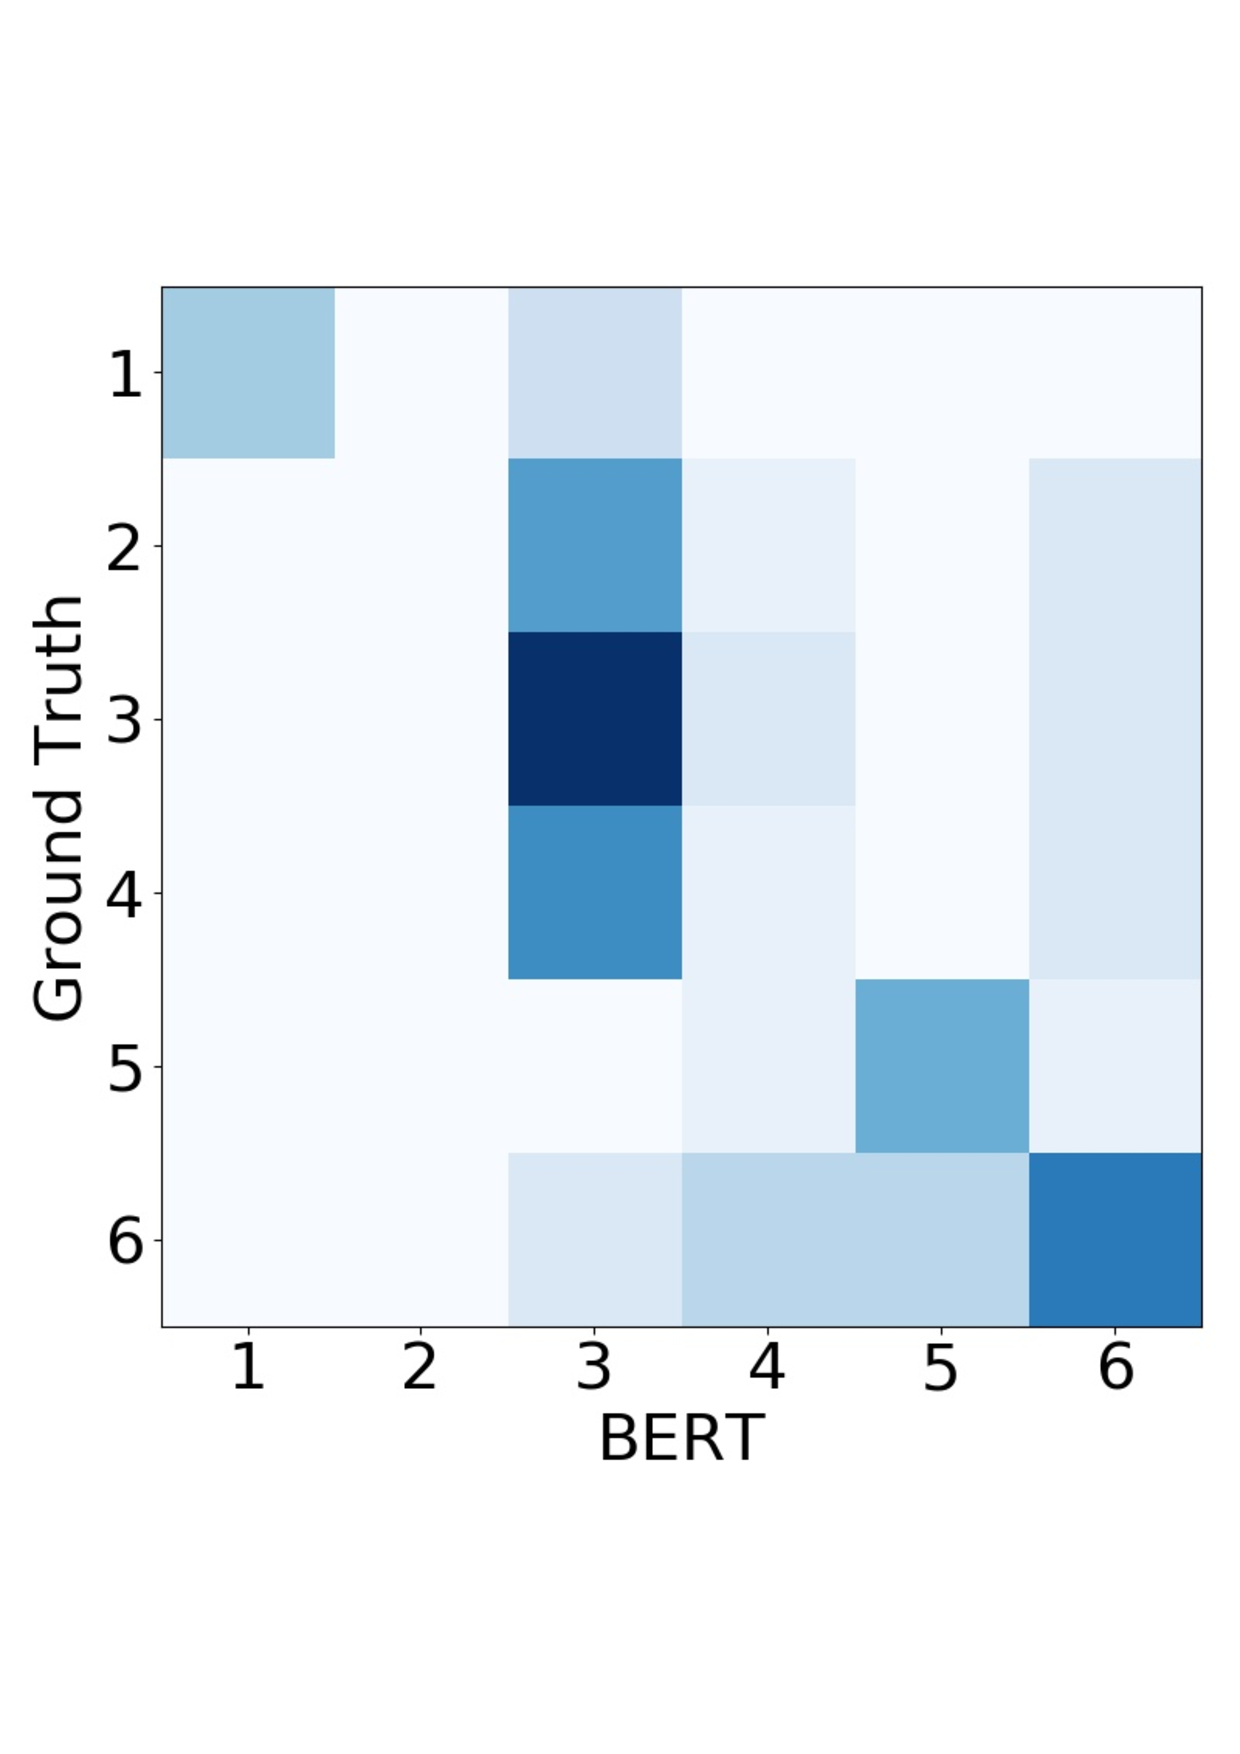
\includegraphics[width=1\linewidth]{BERT_6_pair}\vspace{-1.75cm}
			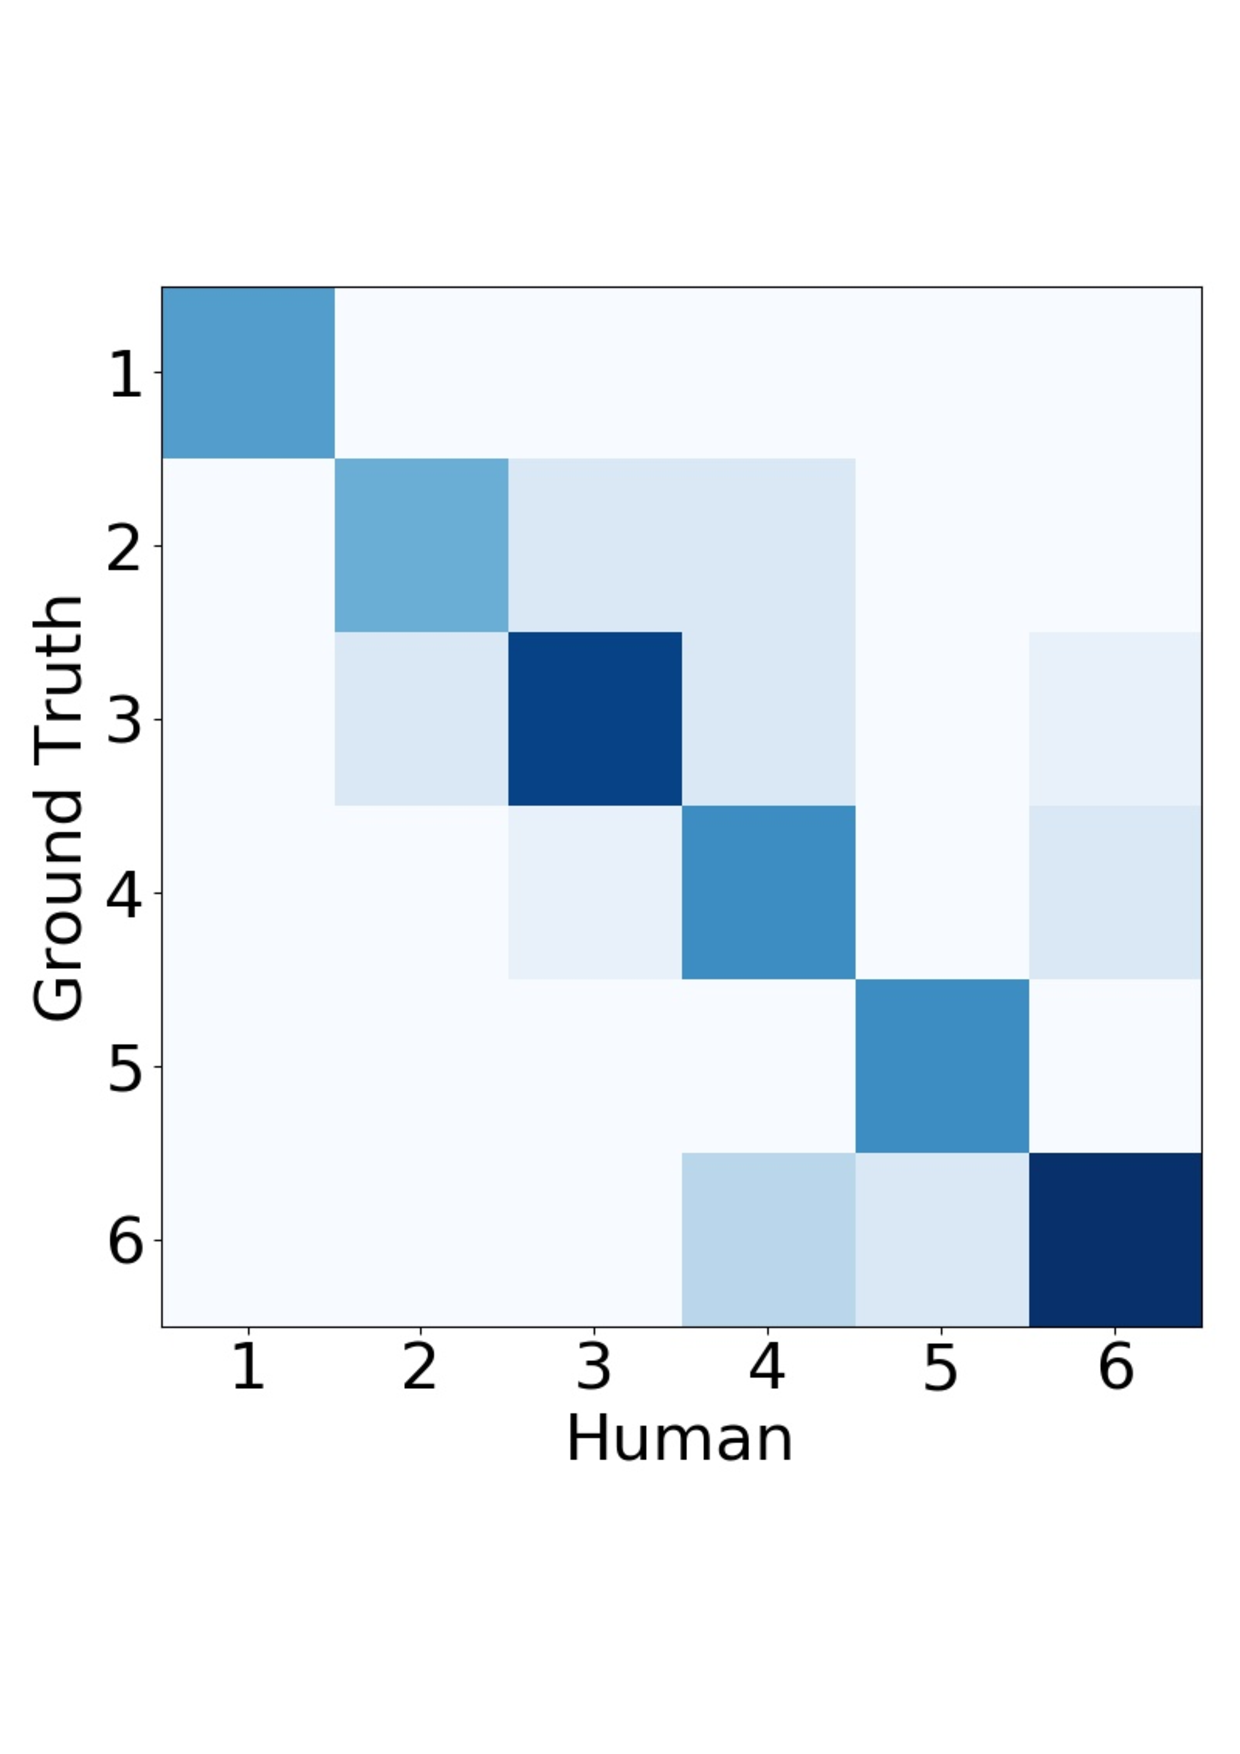
\includegraphics[width=1\linewidth]{human_6_pair}
	\end{minipage}}
	\subfigure{
		\begin{minipage}{0.25\linewidth}
			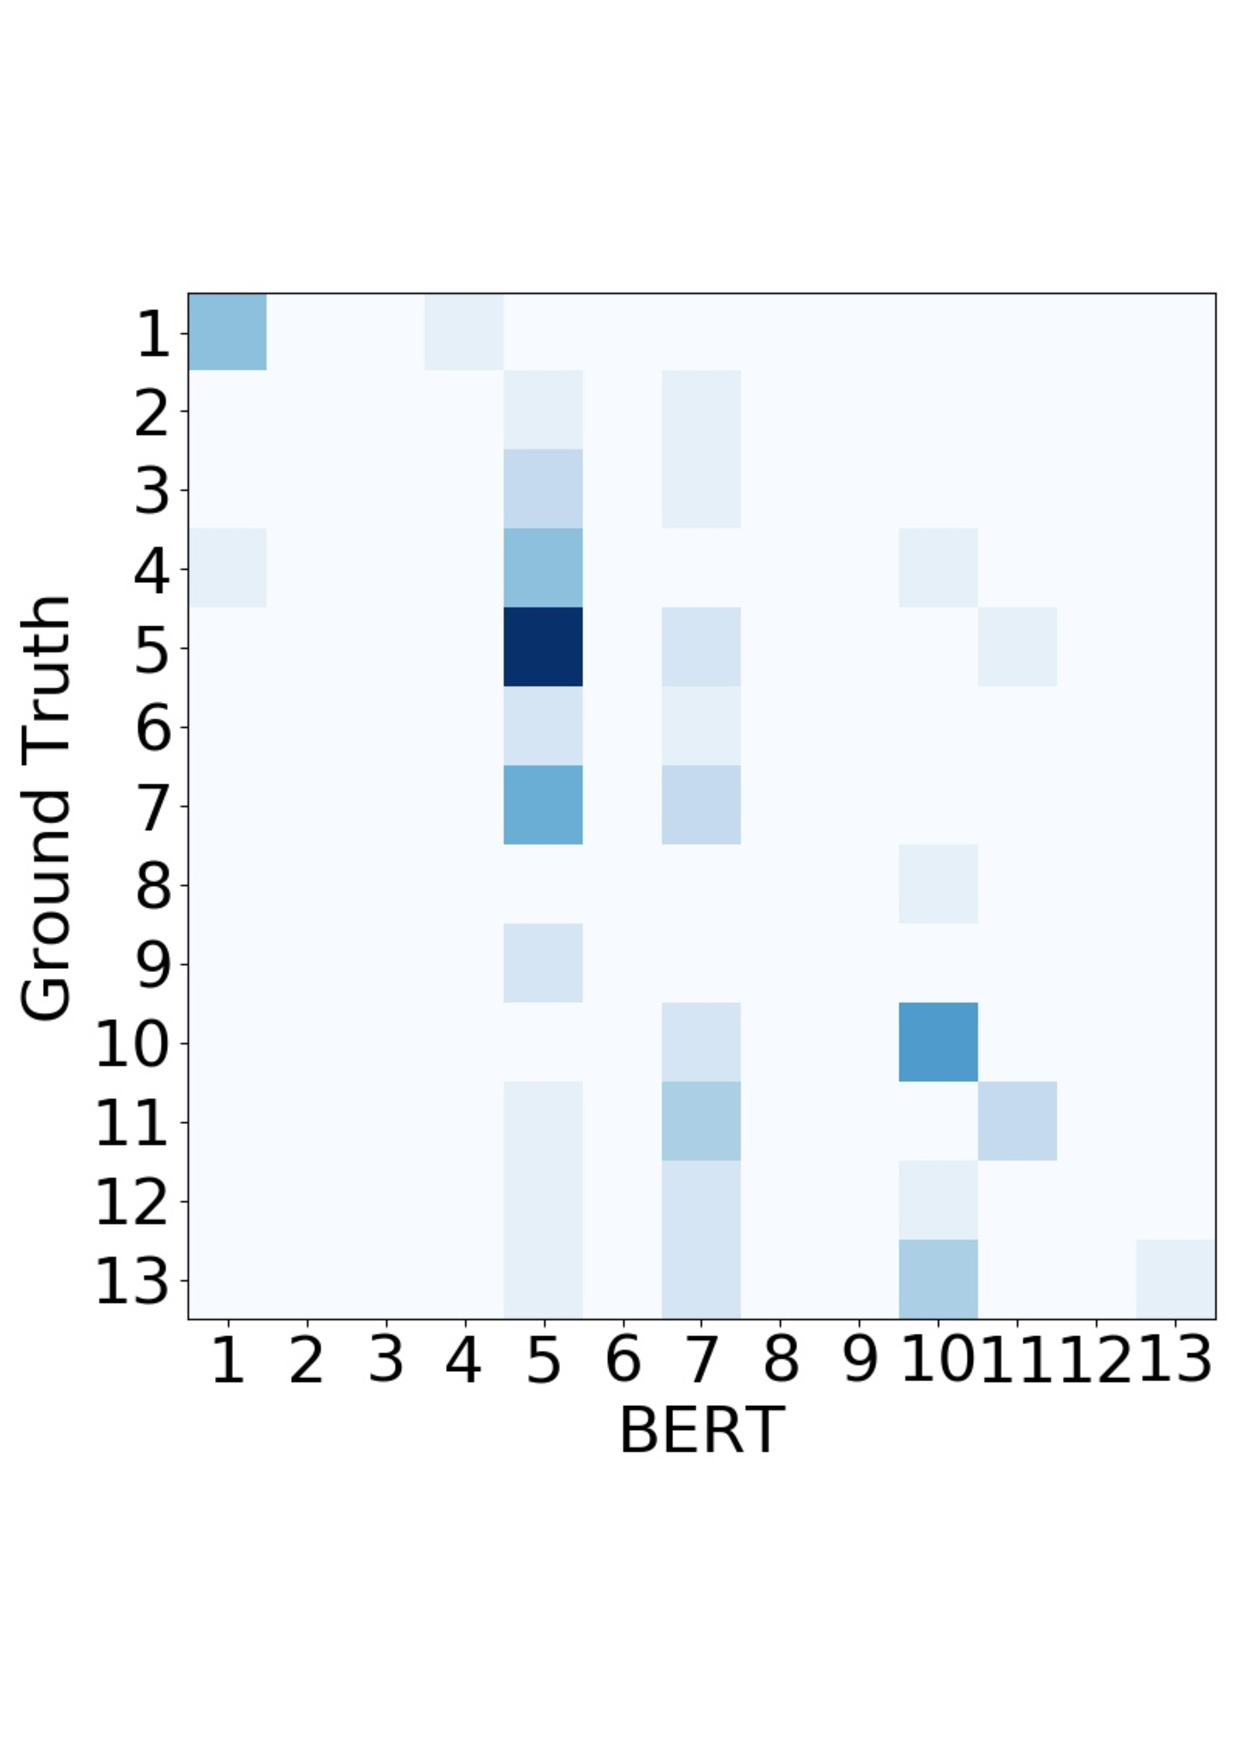
\includegraphics[width=1\linewidth]{BERT_13_pair}\vspace{-1.75cm}
			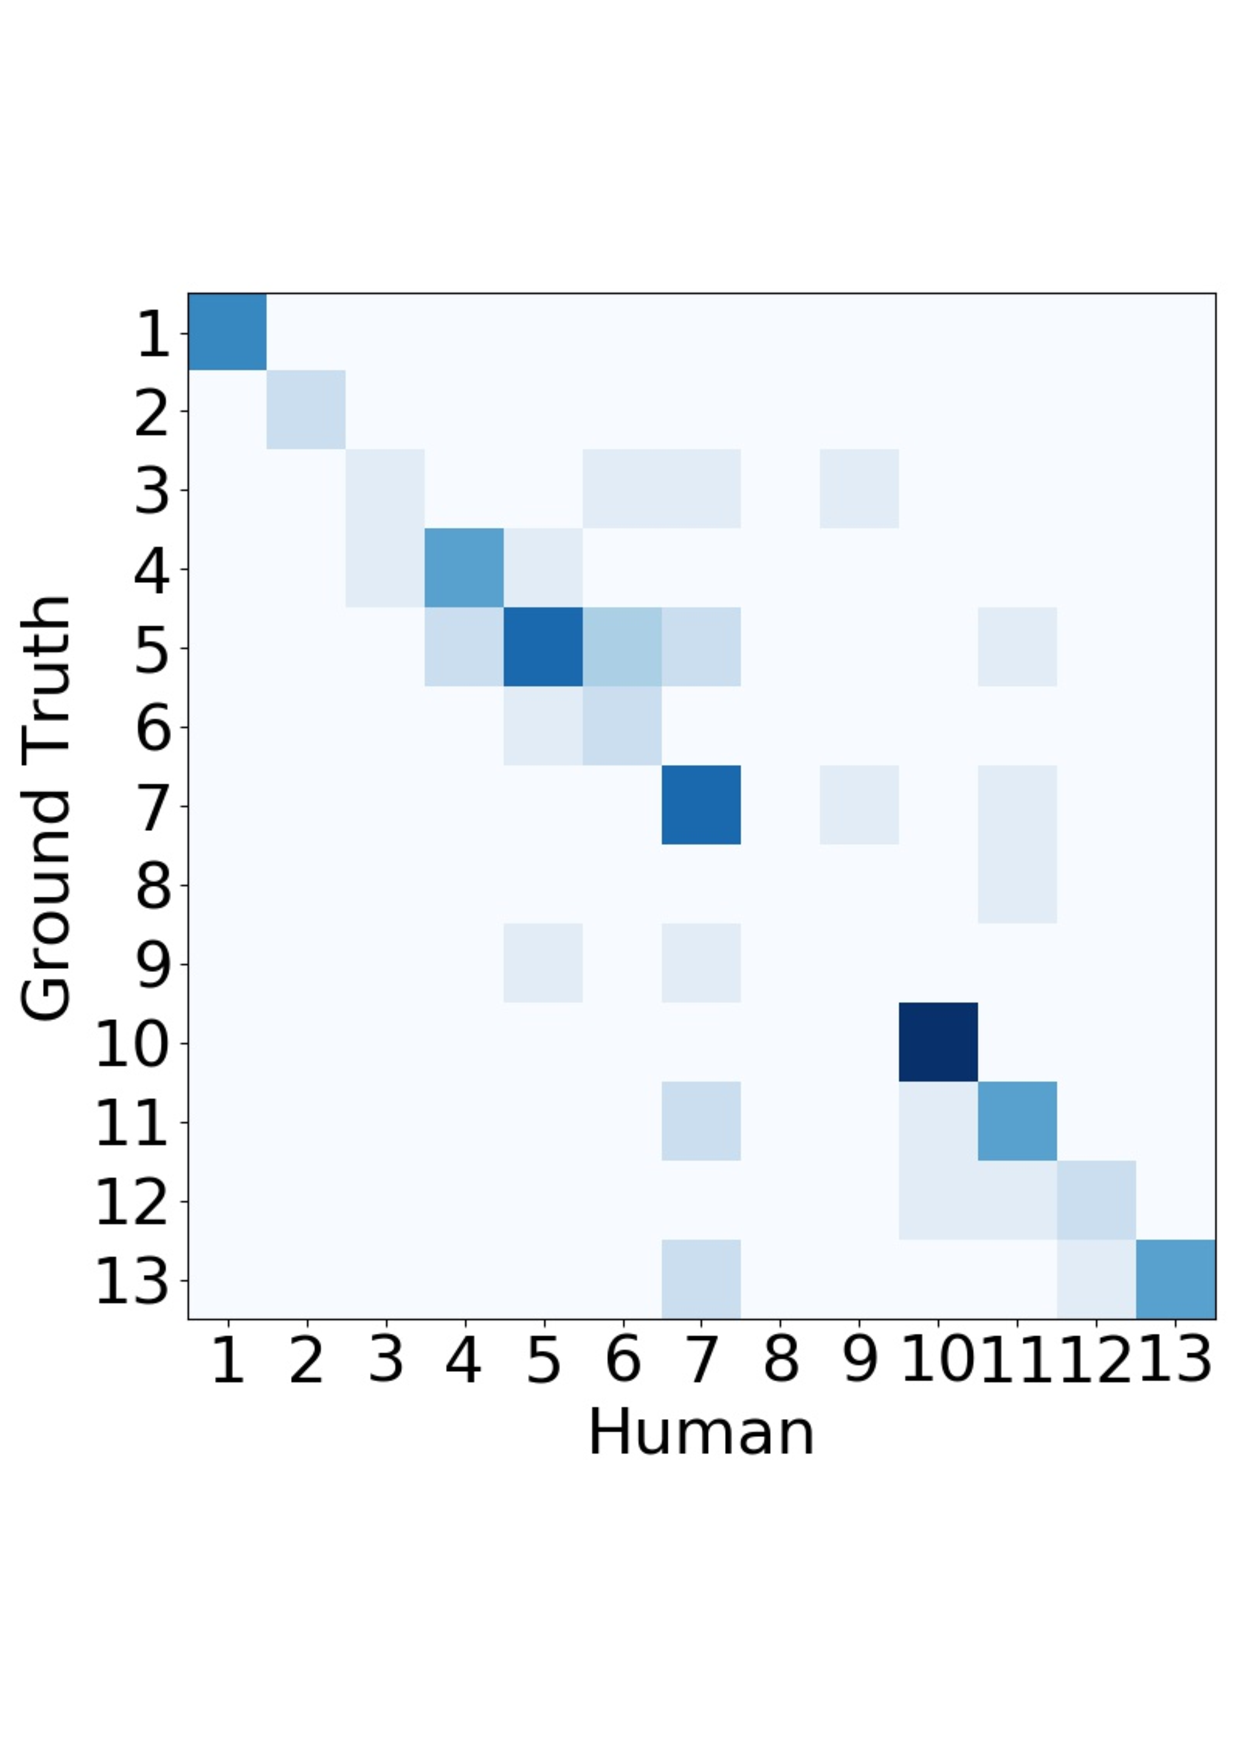
\includegraphics[width=1\linewidth]{human_13_pair}
	\end{minipage}}
	\vspace{-1cm}
	\caption{The confusion matrix of relation classification tasks.}
	\label{fig:confusion}
\end{figure*}
In this section, we discussed both the session-level and pair-level performances with a case study and future directions.
\subsection{Session-level Performance}
We run all of the baseline models with three different random seeds and then obtain the mean and
std value of the evaluation metrics. The results of baselines and human upper bound on session-level relation classification task 
are shown in Table \ref{tab:results}. The difficulties on session-level tasks is in proportional to the number of classes, as the performances of all of the models and human annotators decrease from 4-class task to 13-class task. The gap is about 10\% and 20\% on accuracy for models and human evaluation respectively. 

For Majority baseline, the accuracy is even higher than a neural baseline (LSTM), while the F1-macro is the lowest due to the unbalanced data distribution between classes. The neural baselines almost always performs better than Random and Majority.

The comparison of performances on neural baselines is BERT$>$CNN$>$LSTM. LSTM is much weaker than CNN. The gap between them on 13-class classification is much smaller than 4-class and 6-class classifications due to the fact them both of them failed on fine-grained classification task. The F1-macro is only 4.63\% and 9.20\% respectively with high variance.
BERT, a the pre-trained language model baseline, performs much better and stable than the other two neural models with higher scores and lower variance. The gaps between both evaluation metrics are also much smaller than other baseline, indicating that it can handle the problem of imbalanced data to some extent.

The human performance is the average score of two annotators. We calculate the Cohen's Kappa between them, and the agreement are 0.429, 0.336 and 0.301 for 4-class, 6-class and 13-class relation classification tasks respectively. The agreement on 6-class and 13-class tasks are fair, and on more coarse-grained task, 4-class task, is moderate. It' s also quite difficult for human to identifying the relationship between interlocutors baseline on only one session. It seems that BERT outperforms human upper bound on accuracy of the 13-class classification task, but actually there is no significantly difference between them, and F1-macro score of human upper bound is statistically significant better than BERT with p-value less than 0.05.


%\begin{figure}
	%\centering
	%\subfigure[4-class pair-level results.]{
	% \underline{4-class pair-level results.}\\
	%\vspace{-1cm}
	%\begin{minipage}{0.45\linewidth}
	%	\centering
	%	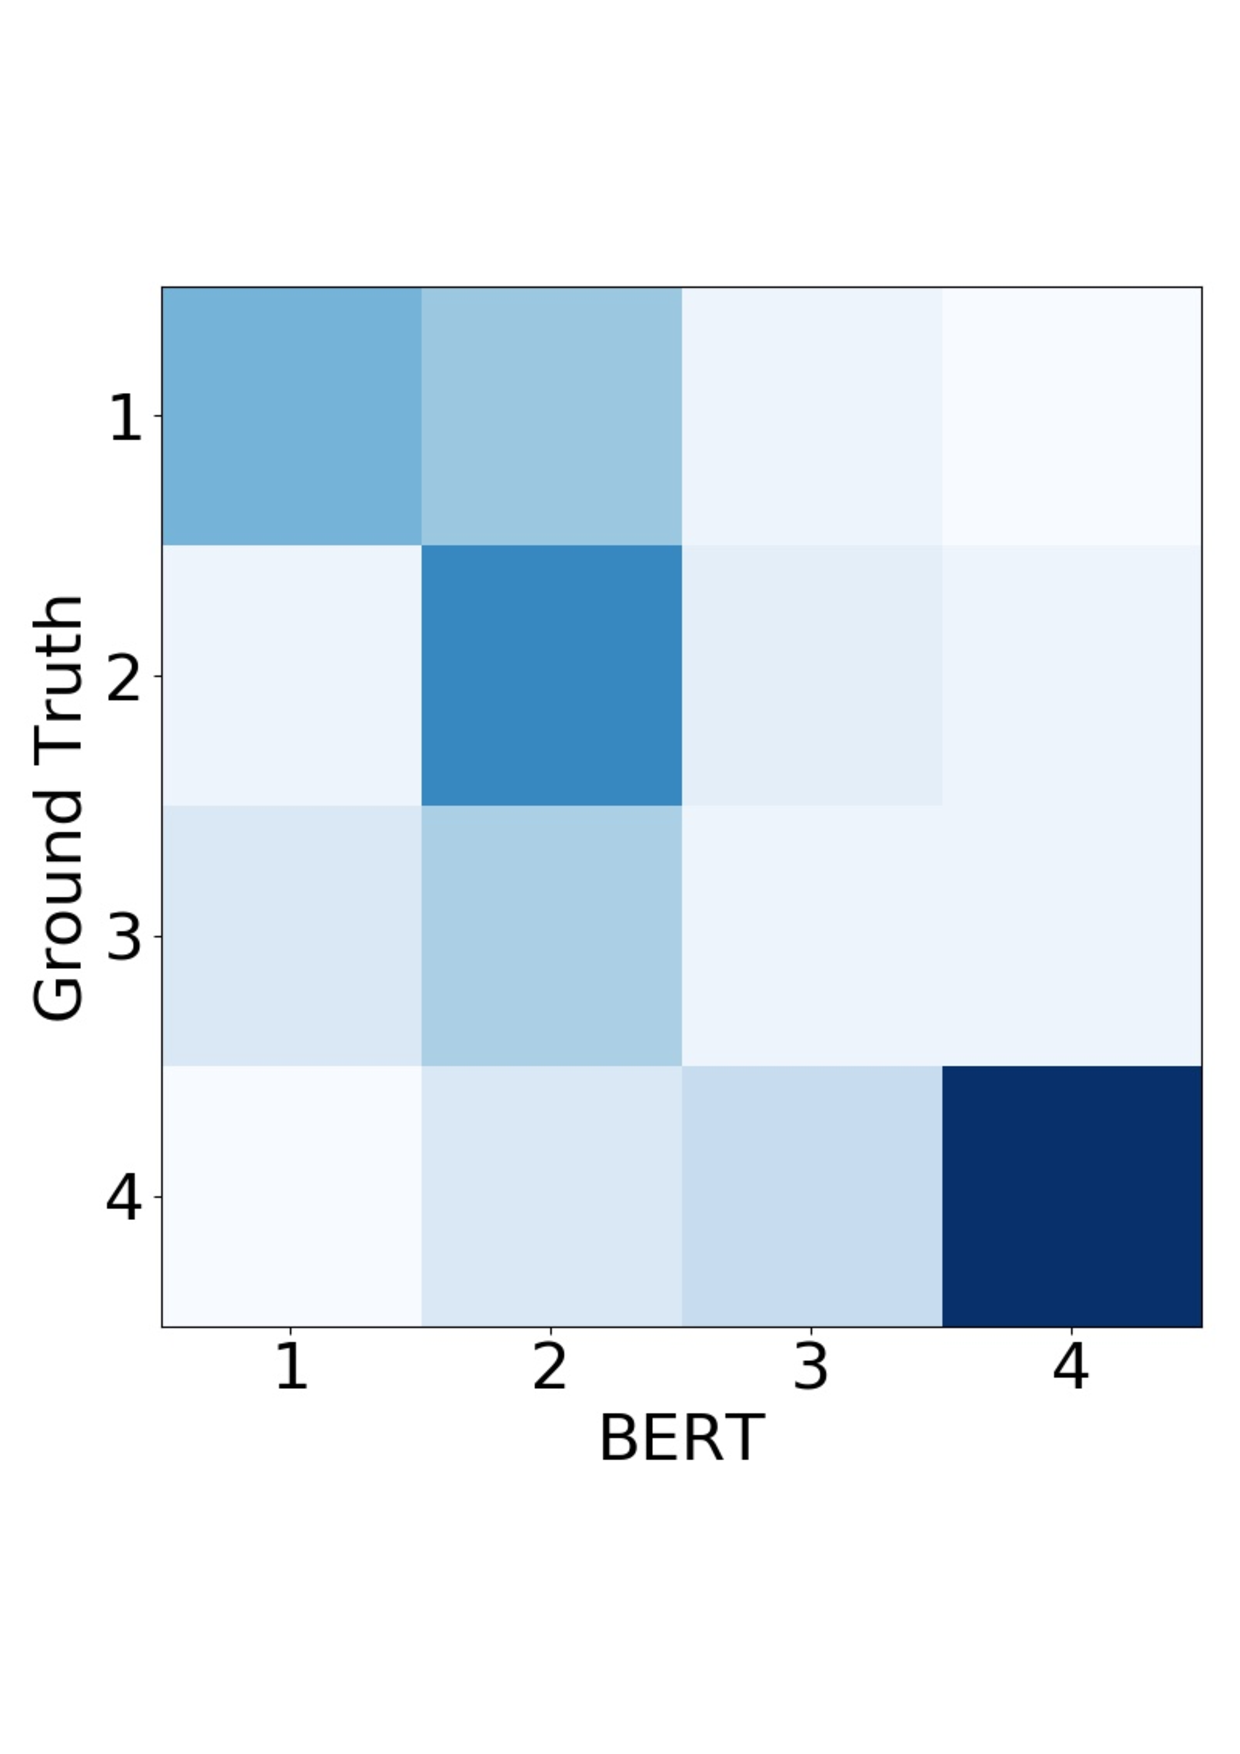
\includegraphics[width=3.8cm]{BERT_4_pair}
	%\end{minipage}
	%\begin{minipage}{0.45\linewidth}
	%	\centering
	%	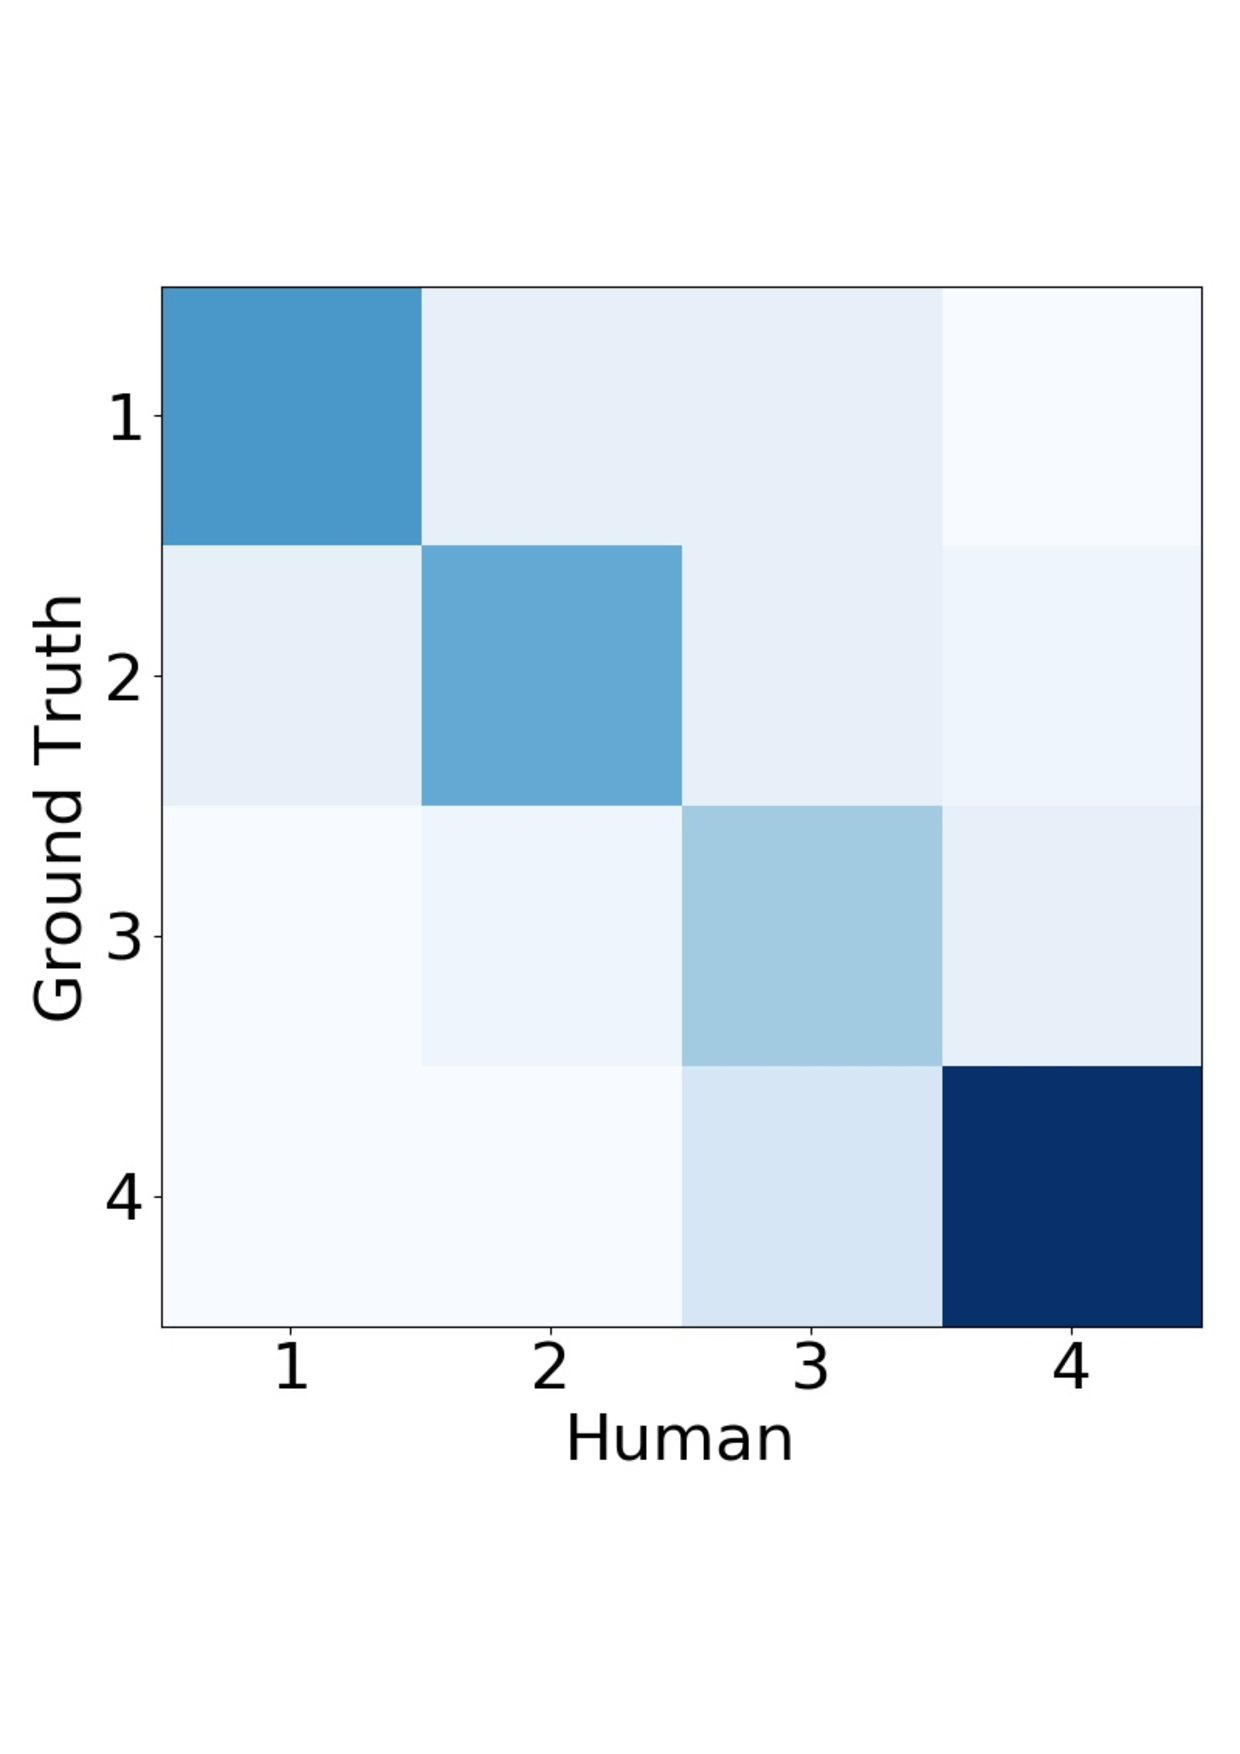
\includegraphics[width=3.8cm]{human_4_pair}
	%\end{minipage}
	% }
%	\vspace{-1cm}
	% \subfigure[6-class pair-level results.]{
%	\begin{minipage}{0.45\linewidth}
%		\centering
%		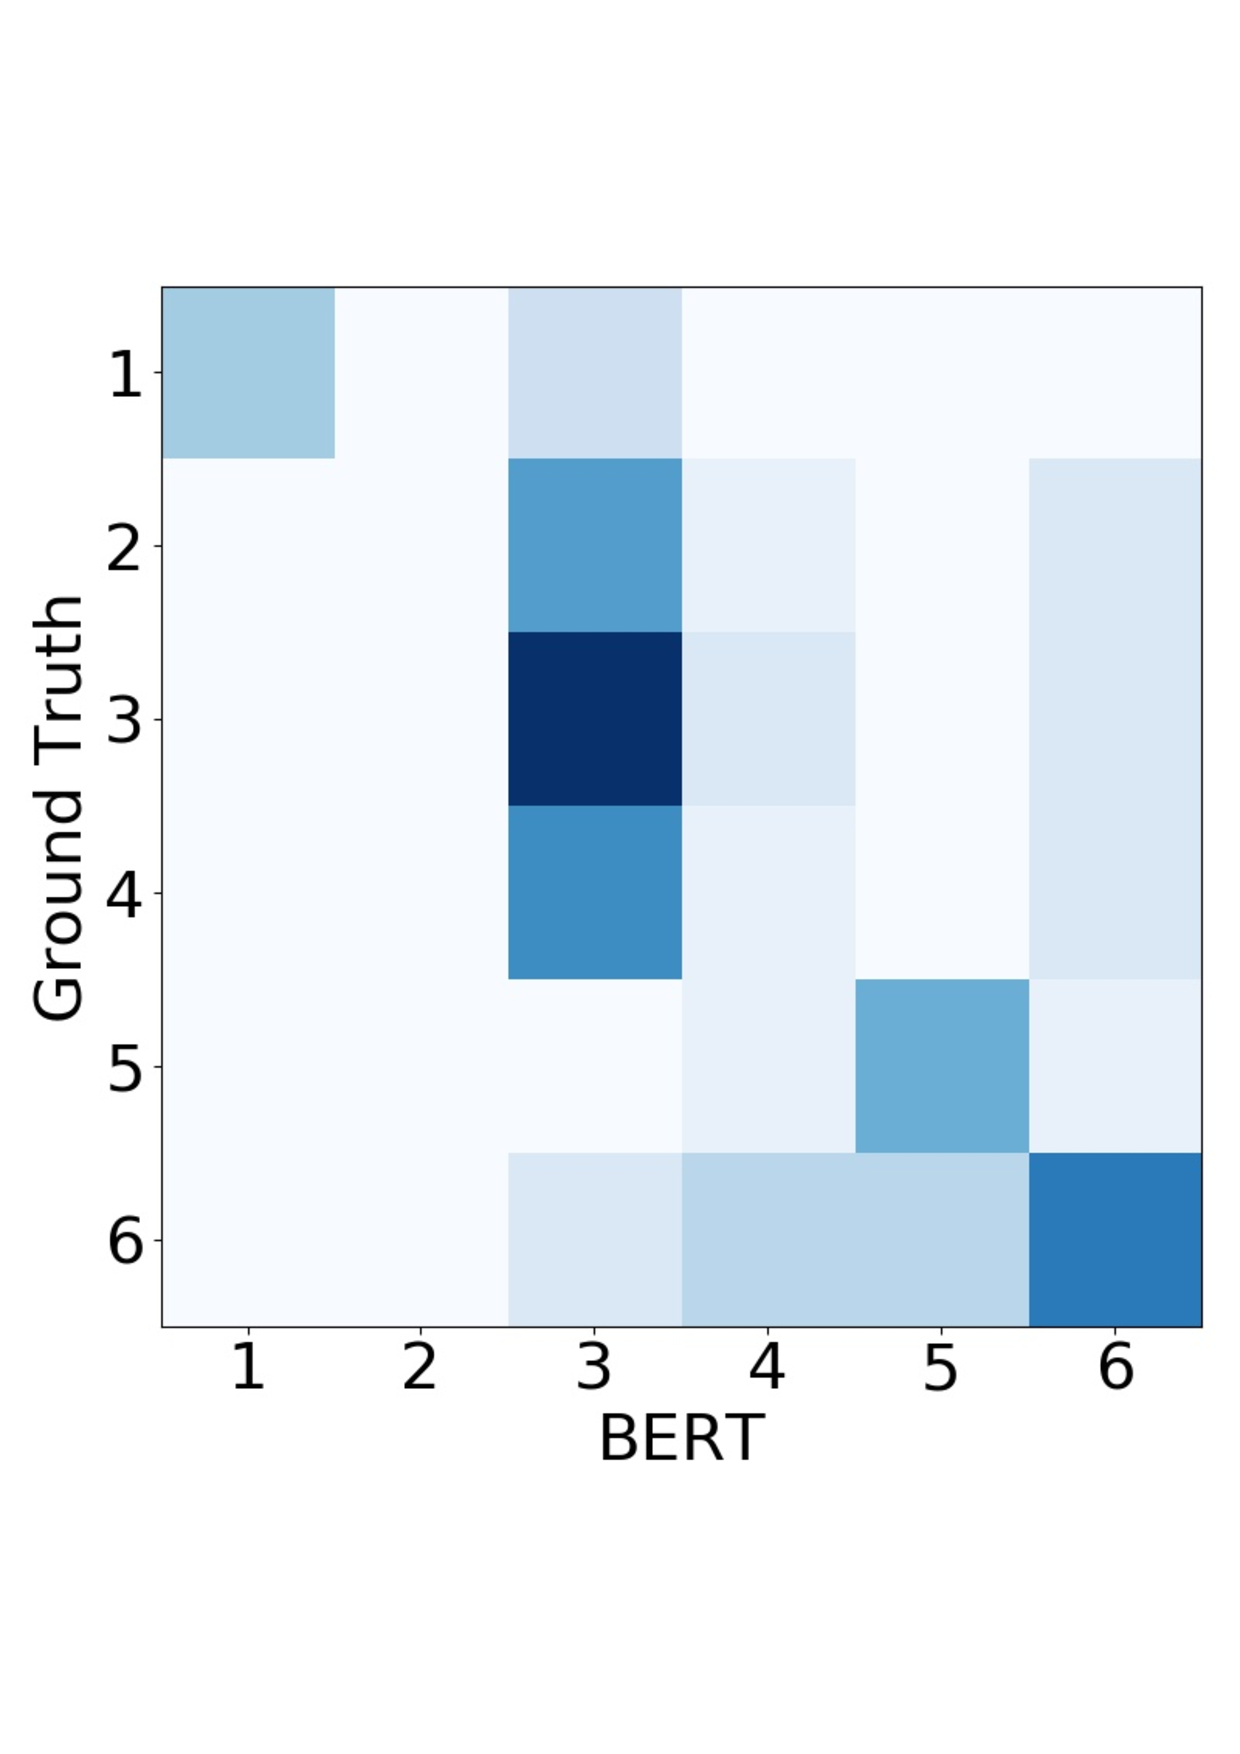
\includegraphics[width=3.8cm]{BERT_6_pair}
%	\end{minipage}
%	\begin{minipage}{0.45\linewidth}
%		\centering
%		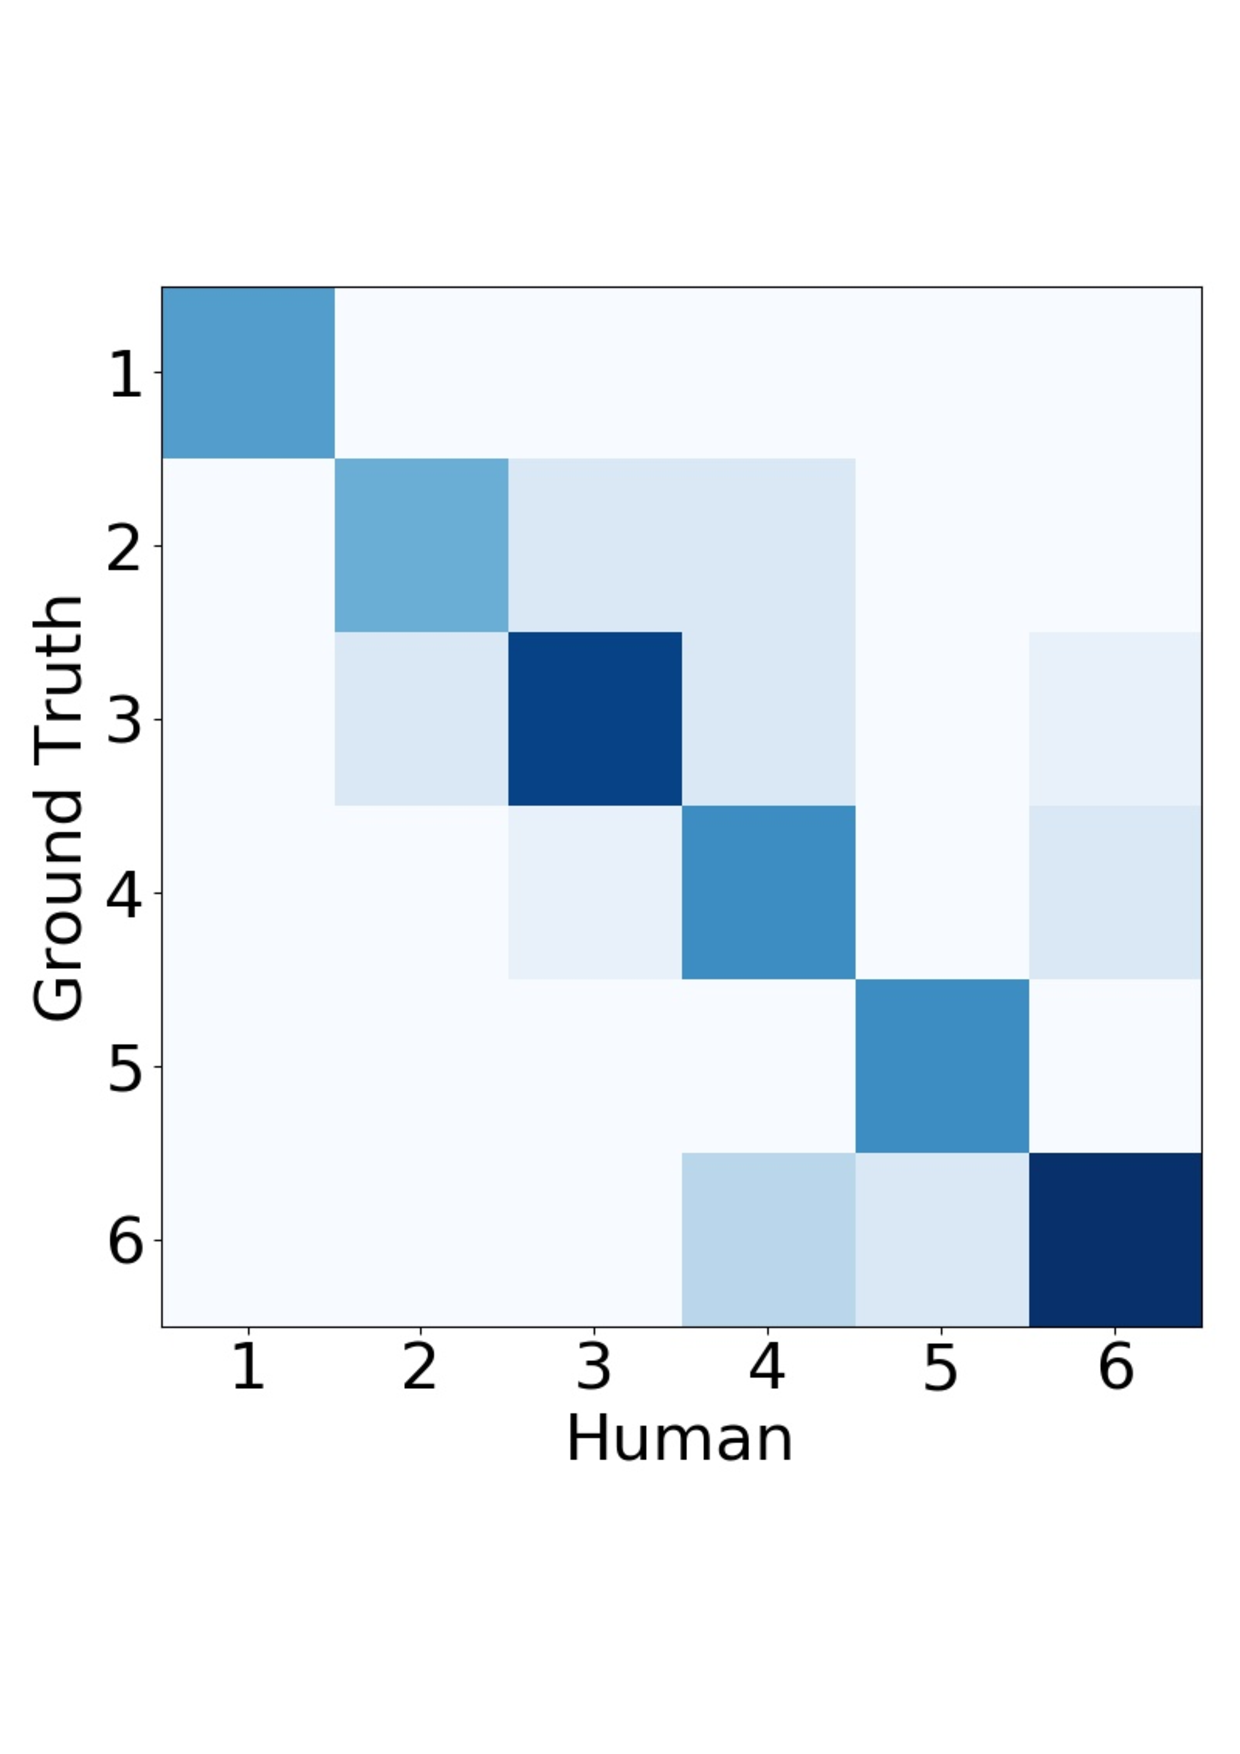
\includegraphics[width=3.8cm]{human_6_pair}
%	\end{minipage}
	% }

%	\vspace{-1cm}
	%\subfigure[13-class pair-level results.]{
%	\begin{minipage}{0.45\linewidth}
%		\centering
%		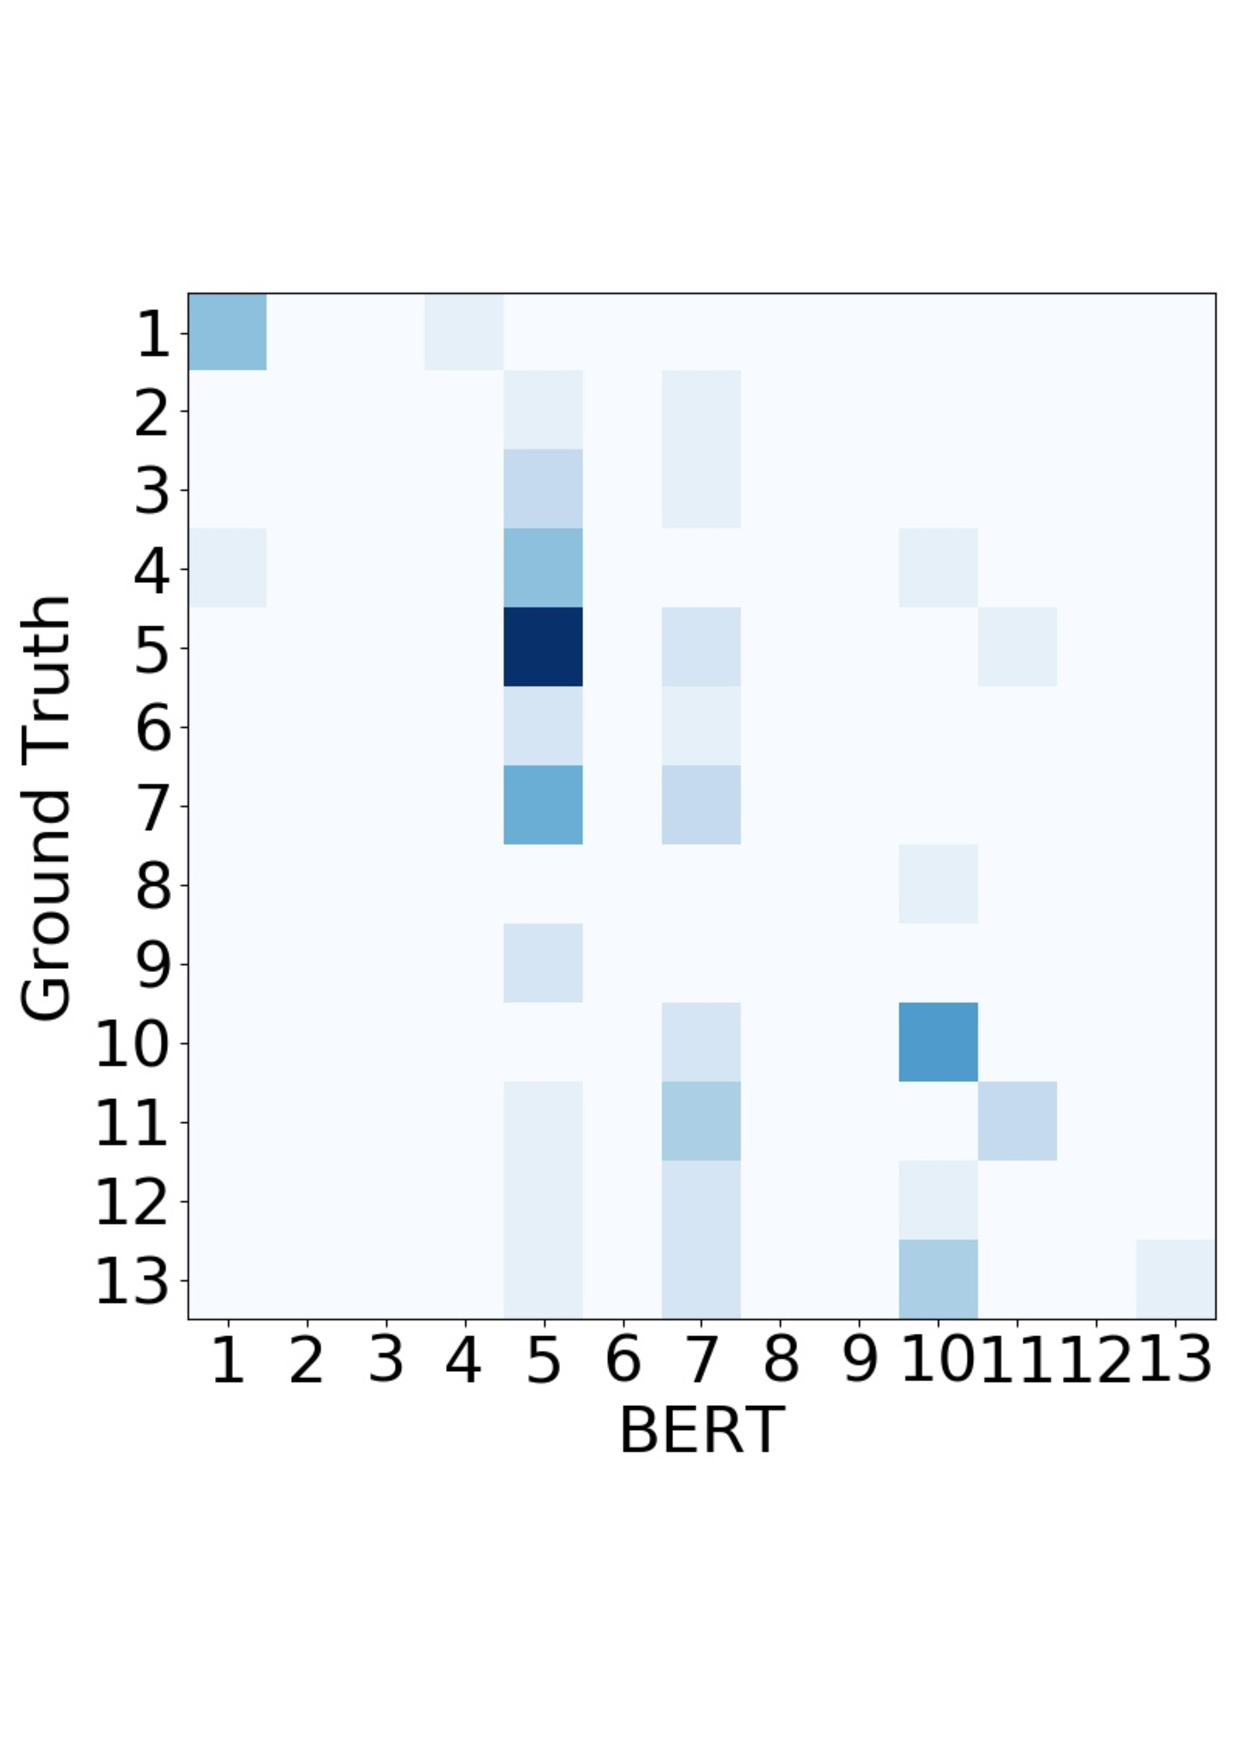
\includegraphics[width=3.8cm]{BERT_13_pair}
%	\end{minipage}
%	\begin{minipage}{0.45\linewidth}
%		\centering
%		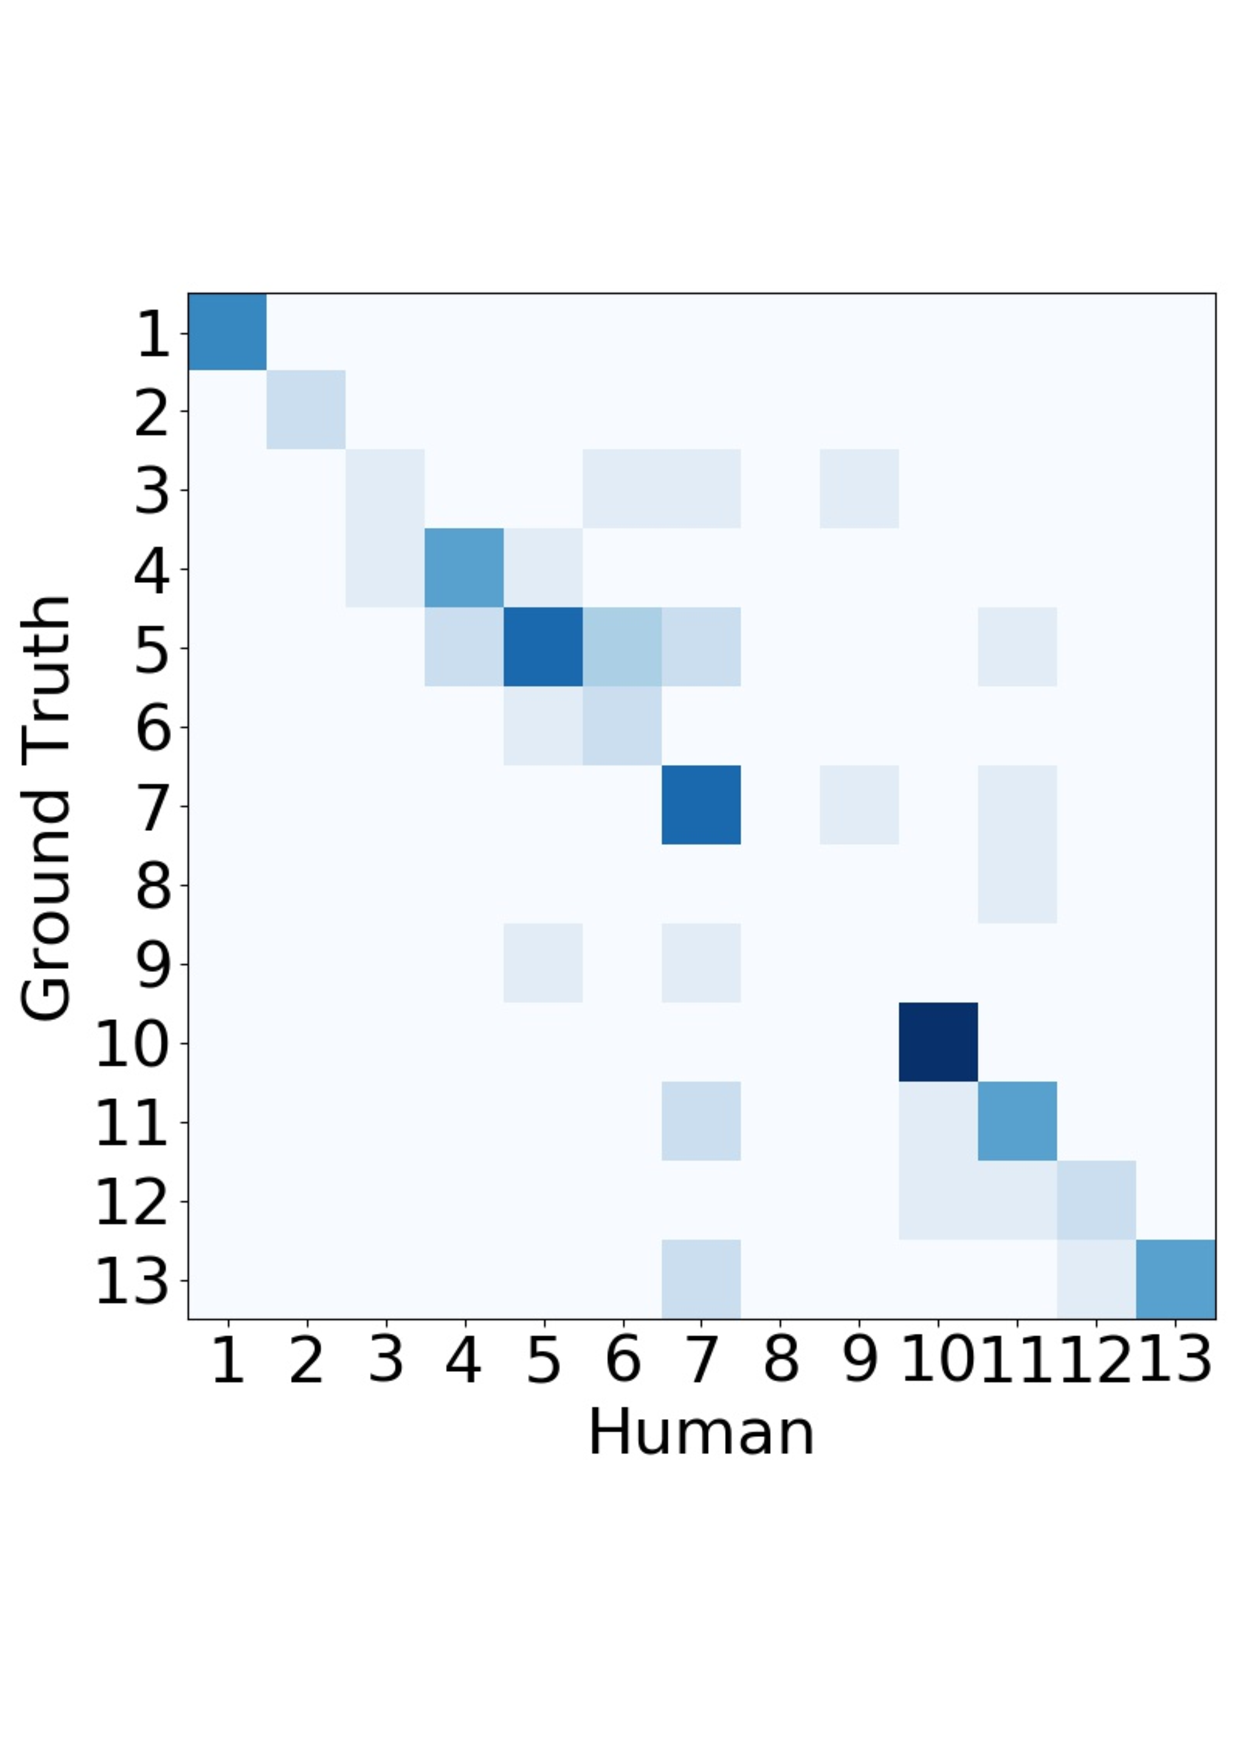
\includegraphics[width=3.8cm]{human_13_pair}
%	\end{minipage}
	%}
%	\caption{The confusion matrix of relation classification tasks.}
%	\label{fig:confusion}
%\end{figure}

% Please add the following required packages to your document preamble:
% \usepackage[table,xcdraw]{xcolor}
% If you use beamer only pass "xcolor=table" option, i.e. \documentclass[xcolor=table]{beamer}

% Please add the following required packages to your document preamble:
% \usepackage[table,xcdraw]{xcolor}
% If you use beamer only pass "xcolor=table" option, i.e. \documentclass[xcolor=table]{beamer}

 \begin{table*}[]
 	\centering
 \begin{tabular}{lcccc}
 \toprule[1.5pt]
 \multicolumn{1}{c}{\textbf{Dialogue Session}}                                                                                                                                                                                                                                    & \textbf{LSTM}                            & \textbf{CNN}                           & \textbf{BERT}                          & \textbf{Human}                           \\ \hline
 \begin{tabular}[c]{@{}l@{}}\textbf{Jim}: All right. All right. I'll listen.\\ ...\\ \textbf{Betsy}: You don't see it, do you, father?\\ \textbf{Jim}: No. Fellow wants to sell a house so he puts an ad in the paper.\\ What did you expect him to do, take it to the United Nations!\end{tabular} & {\color[HTML]{FE0000} Others}   & {\color[HTML]{FE0000} Others} & {\color[HTML]{32CB00} Family} & {\color[HTML]{32CB00} Family}   \\ \hline
 \begin{tabular}[c]{@{}l@{}}\textbf{Jim}: You mean seven-fifteen.\\ \textbf{Betsy}: No, Dad, six-fifteen.\\ ...\\ \textbf{Betsy}: There's a little asterisk. The seven- \\ \textbf{Jim}: Let me see that!\end{tabular}                                                                                              & {\color[HTML]{32CB00} Family}   & {\color[HTML]{32CB00} Family} & {\color[HTML]{32CB00} Family} & {\color[HTML]{32CB00} Family}   \\ \hline
 \begin{tabular}[c]{@{}l@{}}\textbf{Betsy}: You'd better hurry!\\ \textbf{Betsy}: We'll get in a lot of doubles.\\ \textbf{Jim}: Hmm?\\ ...\\ \textbf{Jim}: Uh-huh... Mm-hm. Mm-hm... Uh-huh.\end{tabular}                                                                                                   & {\color[HTML]{FE0000} Intimacy} & {\color[HTML]{FE0000} Others} & {\color[HTML]{FE0000} Others} & {\color[HTML]{FE0000} Intimacy} \\ \hline
 \begin{tabular}[c]{@{}l@{}}\textbf{Jim}: That's none of your business!\\ \textbf{Betsy}: I'd say mother and Uncle Bill were somewhat of an\\ item!\\ \textbf{Betsy}: What about --?\\ \textbf{Jim}: I'll take care of that. Now, shoo, shoo.\end{tabular}                                                   & {\color[HTML]{FE0000} Intimacy} & {\color[HTML]{32CB00} Family} & {\color[HTML]{32CB00} Family} & {\color[HTML]{FE0000} Intimacy} \\ \hline
 \multicolumn{1}{c}{\textbf{Pair Prediction Result}}                                                                                                                                                                                                                              & {\color[HTML]{FE0000} Intimacy} & {\color[HTML]{32CB00} Family} & {\color[HTML]{32CB00} Family} & {\color[HTML]{32CB00} Family}   \\
 \bottomrule[1,5pt]                                                                                                                                                                       
 \end{tabular}
	\caption{The results of a concrete test case. The green labels represent the correct predictions and the red ones are wrong.
 	}
 	\label{case-stduy}
 \end{table*}

% \begin{figure*}
% 	\centering
% 	\includegraphics*[width=0.8\linewidth]{case_study.pdf}
% 	\caption{The results of a concrete test case. The green labels represent the correct predictions and the red ones are wrong.
% 	}
% 	\label{case-stduy}
% \end{figure*}


\subsection{Pair-level Performance}

\label{sec:pair}
Table \ref{tab:results} also included the results on pair-level tasks. The difficulties between classification tasks on different granularity are the same as session-level classification tasks and the comparisons between baseline models are also the same: BERT$>$CNN$>$LSTM. 

By using the MRR metric to get the prediction on pair-level performance of each model as explained in Section \ref{sec:metrics}, it aggravate the polarization of the model performances. The strong baselines like CNN (except on 13-class classification task) and BERT achieve higher scores on pair-level tasks, while others, including LSTM and 13-class CNN model, performs even worse on pair-level tasks. The performance of LSTM is close to Majority baseline. The reason for this phenomenon is that we only assign one label for multiple sessions on pair-level tasks. If the model is weak, it tends to give some extremely unreasonable predictions on some of the sessions for a given pair of interlocutors. Even though there may be some correct predictions on session level, the final prediction for this pair is wrong. On the other hand, if the model is strong, it can give more reasonable predictions for most sessions. Then although there may be some wrong cases on session level, they will be tolerated. The performance of these models will increase.

The gap between CNN and BERT decreases from 4-class to 6-class tasks while increases greatly from 6-class to 13-class tasks. The convolution-based model seems more stable on coarse-grained tasks, and drops dramatically on the 13-class fine-grained task. On the contrary, the performance of fine-tuned language model decreases rapidly from 4-class to 6-class tasks and decreases slowly from 6-class to 13-class tasks. As a result, the advantage of BERT model on 6-class classification tasks is limited beyond the CNN baseline.

The human also performances much better on pair-level tasks than session-level tasks. The Cohen's Kappa for two annotators are 0.698, 0.687 and 0.614 for 4-class, 6-class and 13-class relation classification tasks respectively, showing substantial agreements. The higher performances and agreement is consistent with the intuition that, with multiple sessions for a given pair, human are able to find more correlations between sessions and better understand the background of two interlocutors. In this way, we think that pair-level relation classification tasks are more reasonable, challenging and meaningful for the development of current models. 

The gap between best baseline BERT and Human performances also showing the limitation of current models. We draw the confusion metrics for the best neural model BERT and human performances in Figure \ref{fig:confusion}. We can see that for coarse-level relation classification tasks, the performance of BERT and human has some similarities. They both did well on predicting the official relation type on 4-level task, and intimacy-peer relation type and official-peer relation type on 6-level task. For 13-classification tasks, BERT fails dramatically which may due to the unbalanced data distribution, tending to predict the relation type of "{\em lovers}", while human performance well on the relation type of "{\em Workplace Superior-Subordinate}".




\subsection{Case Study}
We present a concrete case study of 4-class classification task in Table \ref{case-stduy}. There are 4 sessions
in this pair of speakers. In some of the session, we can see word \textit{dad} that 
strongly indicates the relation between the speakers should be \{\textit{child-parent}\}.
Except LSTM, all of the models can capture this indicator and therefore correctly
predict the relation for those sessions. We can also see that even human cannot give the 
correct relation for all of the session. However, based on MMR metric, most of the models
can still predict the correct relation for the pair of speakers.



\subsection{Future Directions}

We consider the further research on this task as follows:

\textbf{Cross-session Consideration.} As talked about in Section \ref{sec:pair}, classification of a pair of interlocutors based on multiple sessions between them is a more reasonable and meaningful tasks. Due to the fact that the number of sessions for pairs varies a lot and it's difficult and unreasonable to concatenate all of the utterances in these sessions as the input for models, we only combines the prediction results of each session to get the final pair-level predictions. However, cross-session consideration is important. Developing models that could better find the cues between sessions is an important direction for current models.

\textbf{Commonsense Knowledge.} Another limitation of current models is due to the lack of commonsense knowledge, even for commonly pre-trained language models. Human can better inference the background of two interlocutors with the previous stories or experiences they have had. Further pre-training the language models on more similar corpus and incorporating the commonsense knowledge base, such as ConceptNet~\cite{SpeerCH17}, are possible solutions.